\chapter{Технологический раздел}
\section{Выбор среды разработки}

В качестве основной технологии для разработки серверной части системы выбран
язык высокого уровня \Soft{Python} и набор инструментов для построения веб-приложений
\Soft{Django}.

На выбор языка оказали влияние следующие факторы:

\begin{enumerate}
\item Ясность и читаемость кода как следствие синтаксических особенностей языка;
\item Возможность создания модульный программ, поддержка иерархии пакетов;
\item Поддержка основных возможностей функционального программирования, а также
полная поддержка парадигмы ООП;
\item Высокоуровневые типы данных;
\item Динамическая типизация;
\item Большое количество стандартных библиотек и функций;
\item Язык подходит для прототипирования;
\item Наличие библиотек для работы с численными массивами и матричных вычислений
(NumPy, SciPy), а также дополнительных утилит для обработки сигналов, позволяет
использовать Python в качестве альтернативы таким системам, как MatLab;
\item Свободная лицензия позволяет использовать язык для создания как свободных,
так и проприетарных приложений.
\end{enumerate}

На выбор \Soft{Django} для построения серверной части комплекса повлияли
следующие факторы:

\begin{enumerate}
\item Использование данного ПО для реализации целевой системы (системы
управления студенческими проектами кафедры ИУ-7 МГТУ им.~Н.~Э.~Баумана);
\item Использование \Code{Python} в качестве языка программирования. \Code{Python} предоставляет мощные средства метапрограммирования, обширную библиотеку классов, хорошую документацию;
\item Полная документация. Вместе с \Code{Django} поставляется качественная документация с подробным объяснением основных концепций, множество примеров;
\item Встроенный ORM (\important{Object-relational mapper}). Обеспечивает проецирование реляционных данных в объекты, благодаря чему в большинстве случаев совершенно не требуется использование SQL-синтаксиса в выражениях, что автоматически снижает риск появления \Code{SQL-injection} уязвимости;
\item Поддержка \Code{MTV} (\Code{Model-Template-View}). Данный паттерн проектирования очень близок к классическому \Code{MVC}, позволяет отделять бизнес-логику от дизайна;
\item Высокая скорость работы. \Code{Django} может выдерживать высокую нагрузку, так как имеет встроенные средства кэширования и распределения нагрузки;
\item Предоставление прототипов для развертывания административной части системы.
\end{enumerate}

Для реализации очередей запросов выбран протокол \Soft{AMQP} (Advanced Message
Queuing Protocol) и его серверная реализация на языке \Soft{Erlang}~---
\Soft{RabbitMQ}.

Для реализации функционала на стороне клиента использован HTML/JavaScript. Для
работы с микрофоном, записи и отправки голосовых данных на
сервер используется Java-апплет. Решено использовать Java по следующим причинам:

\begin{enumerate}
\item На сегодняшний день единственной альтернативой встраивания Java для
доступа к микрофону пользователя из браузера является технология Flash или
создание зависящих от браузера дополнений;
\item При использовании Flash появляется необходимость использования
проприетарного приложения Flash Media Server для получения данных от
пользователя;
\item Среда исполнения Java доступна на большинстве существующих
программно-аппаратных платформ, в том числе мобильной платформе Windows Mobile
6, апплеты широко распространены, поэтому снижается требовательность системы к
конфигурации пользовательской ЭВМ.
\end{enumerate}

\section{Описание программы}
\subsection{Общие сведения}
\label{sec:soft_description:general}

Для функционирования программы необходимо следующее программное обеспечение:
\begin{itemize}
\item Python 2.6.2;
\item SciPy 0.7.2 с набором инструментов \Soft{scikits} (\url{http://scikits.appspot.com}, 2010);
\item NumPy 1.4.1;
\item Django 1.1.1;
\item Apache 2.2.14 с модулем mod\_python или wsgi (или другой веб-сервер,
поддерживающий интерфейс WSGI);
\item RabbitMQ 1.5.4 (\url{http://www.rabbitmq.com}, 2010);
\item GNU Make 3.81;
\item Поддерживаемая Django СУБД: PostgreSQL версии 8.2 или выше, MySQL 4.1/5.0, Oracle версии 9i или выше, SQLite версии 3.3.6 или выше; возможно использование других СУБД при наличии соответствующего интерфейса (см.~\url{http://docs.djangoproject.com/en/dev/ref/databases/#using-a-3rd-party-database-backend}, 2010);
\end{itemize}

Программа написана полностью на языке \Soft{Python} (\url{http://www.python.org}, 2010) с использованием веб-фреймворка \Soft{Django} (\url{http://www.djangoproject.com}, 2010), библиотеки для работы с многомерными массивами \Soft{NumPy} и библиотеки научных инструментов \Soft{SciPy} (\url{http://www.scipy.org}, 2010). Все вышеперечисленное ПО (за исключением СУБД Oracle) является свободным и кроссплатформенным.

\subsection{Функциональное назначение}

Программный комплекс предназначен для голосовой аутентификации пользователя
интернет-сайта.

Основные функциональные возможности:
\begin{itemize}
\item Создание персональной модели голоса пользователя, позволяющей
аутентифицировать его по ключевой фразе;
\item Вход в защищаемый раздел интернет-ресурса по ключевой фразе, используемой
при регистрации;
\item Возможность настройки параметров чувствительности системы;
\item Возможность добавления, просмотра и редактирования параметров и сущностей
системы через интерфейс администратора;
\item Ведение системного журнала событий;
\item Возможность встраивания в существующий интернет-портал, использующий
технологию Django.
\end{itemize}

\subsection{Описание логической структуры}

В данном разделе дано описание основных модулей программного комплекса.

\subsubsection*{Структура модулей системы}

%На рисунке~\ref{fig:package_tree} представлена иерархия модулей системы.

%\begin{figure}[ht]
%\center{\scalebox{1.0}{\begin{tikzpicture}[text height=0.7em,text depth=0.25ex]
    \tikzset{
        >=latex',
        ordnode/.style = draw,fill=gray!10,shape=rectangle,
    }

    \small\ttfamily{
    \begin{dot2tex}[dot,tikz,styleonly]
        \begin{tikzpicture}[text height=0.7em,text depth=0.25ex]
    \tikzset{
        >=latex',
        ordnode/.style = draw,fill=gray!10,shape=rectangle,
    }

    \small\ttfamily{
    \begin{dot2tex}[dot,tikz,styleonly]
        \begin{tikzpicture}[text height=0.7em,text depth=0.25ex]
    \tikzset{
        >=latex',
        ordnode/.style = draw,fill=gray!10,shape=rectangle,
    }

    \small\ttfamily{
    \begin{dot2tex}[dot,tikz,styleonly]
        \input{dot/package_tree.dot}
    \end{dot2tex}
    }
\end{tikzpicture}


    \end{dot2tex}
    }
\end{tikzpicture}


    \end{dot2tex}
    }
\end{tikzpicture}

}}
%\label{fig:package_tree}
%\caption{Иерархия модулей системы}
%\end{figure}

На рисунке~\ref{fig:import_graph} представлена иерархия модулей системы по
отношению взаимного использования. Модули
пакета \Code{verispeak}, который представляет собой реализацию библиотеки
инструментов для голосовой аутентификации, детально рассмотрены далее.

\begin{figure}[ht!]
\center{\scalebox{0.77}{\begin{tikzpicture}[text height=0.7em,text depth=0.25ex]
    \tikzset{
        >=latex',
        ordnode/.style = draw,fill=gray!10,shape=rectangle,
    }

    \small\ttfamily{
    \begin{dot2tex}[dot,tikz,styleonly]
        \begin{tikzpicture}[text height=0.7em,text depth=0.25ex]
    \tikzset{
        >=latex',
        ordnode/.style = draw,fill=gray!10,shape=rectangle,
    }

    \small\ttfamily{
    \begin{dot2tex}[dot,tikz,styleonly]
        \begin{tikzpicture}[text height=0.7em,text depth=0.25ex]
    \tikzset{
        >=latex',
        ordnode/.style = draw,fill=gray!10,shape=rectangle,
    }

    \small\ttfamily{
    \begin{dot2tex}[dot,tikz,styleonly]
        \input{dot/import_graph.dot}
    \end{dot2tex}
    }
\end{tikzpicture}


    \end{dot2tex}
    }
\end{tikzpicture}


    \end{dot2tex}
    }
\end{tikzpicture}

}}
\caption{Граф импортирования модулей системы (контроллер)}
\label{fig:import_graph}
\end{figure}

Модули контроллера соответствуют соглашениям и требованиям используемого
инструментария \Soft{Django}:
\begin{itemize}
\item \Code{views}~--- модуль, содержащий определения всех ресурсов системы
аутентификации,
предоставляемых сервером внешним клиентам;
\item \Code{models}~--- модуль, определяющий сущности системы в виде классов,
которые отображаются в базу данных;
\item \Code{forms}~--- модуль, содержащий классы, которые представляют
HTML-формы;
\item \Code{views.enrollment}~--- подмодуль, содержащий определения ресурсов,
относящихся к стадии регистрации (обучения модели);
\item \Code{views.verification}~--- подмодуль, содержащий определения ресурсов,
онтосящихся к стадии аутентификации;
\item \Code{services}~--- в данном модуле определены обработчики заявок на
обучение модели и аутентификацию. Это единственный модуль контроллера, который
связан с библиотекой функций для голосовой аутентификации (через
\Code{verispeak.api});
\item \Code{amqp}~--- клиент для протокола обмена сообщениями AMQP, позволяющий
ставить заявки на обучение модели и аутентификацию, код обработчиков которых
находится в модуле \Code{services};
\item \Code{ip}~--- вспомогательный модуль, используемый для преобразования
строкового представления IP-адреса клиента в упакованный вид (целое число) и
обратно;
\item \Code{signature}~--- вспомогательный модуль, определяющий функции для
подписывания данных секретным ключом (используется при генерации уникального
идентификатора сессии в сессиях регистрации и аутентификации);
\item \Code{state\_machine.models}~--- в данном модуле определен базовый класс
для реализации сущностей, обладающих состояниями (процесс аутентификации и
процесс обучения модели).
\end{itemize}

\begin{figure}[htp!]
\scalebox{0.75}{
\begin{sideways}
\begin{tikzpicture}[text height=0.7em,text depth=0.25ex]
    \tikzset{
        %>=latex',
        ordnode/.style = draw,fill=gray!10,shape=rectangle,
        last/.style = draw,fill=gray!20,shape=rectangle,
    }

    \small\ttfamily{
    \begin{dot2tex}[dot,tikz,styleonly]
        \begin{tikzpicture}[text height=0.7em,text depth=0.25ex]
    \tikzset{
        %>=latex',
        ordnode/.style = draw,fill=gray!10,shape=rectangle,
        last/.style = draw,fill=gray!20,shape=rectangle,
    }

    \small\ttfamily{
    \begin{dot2tex}[dot,tikz,styleonly]
        \begin{tikzpicture}[text height=0.7em,text depth=0.25ex]
    \tikzset{
        %>=latex',
        ordnode/.style = draw,fill=gray!10,shape=rectangle,
        last/.style = draw,fill=gray!20,shape=rectangle,
    }

    \small\ttfamily{
    \begin{dot2tex}[dot,tikz,styleonly]
        \input{dot/import_graph_verispeak.dot}
    \end{dot2tex}
    }
\end{tikzpicture}


    \end{dot2tex}
    }
\end{tikzpicture}


    \end{dot2tex}
    }
\end{tikzpicture}


\end{sideways}
}
\caption{Граф импортирования модулей системы (библиотеки голосовой
аутентификации)}
\label{fig:import_graph_verispeak}
\end{figure}

Опишем модули библиотеки инструментов для голосовой аутентификации, граф
импортирования которых представлен на представлены на
рисунке~\ref{fig:import_graph_verispeak}:

\begin{itemize}
\item \Code{model}~--- модуль содержит определения классов, предназначенных для
моделирования источника речи;
\item \Code{model.base}~--- модуль, в котором содержится определение базового
класса \Code{Codebook};
\item \Code{model.gmm}~--- модуль содержит реализации \Code{Codebook},
основанные на гауссовых смесях;
\item \Code{model.gmm.base}~--- определение базового класса \Code{GmmBase};
\item \Code{model.gmm.full\_gmm}~--- определение класса \Code{FullGMM};
\item \Code{model.gmm.diagonal\_gmm}~--- определение класса \Code{DiagonalGMM};
\item \Code{stats.mvn}~--- модуль содержит различные функции для работы с
многомерным нормальным распределением: нахождение значения функции плотности
распределения в некоторой точке многомерного пространства;
\item \Code{training}~--- модуль содержит определения классов, предназначенных
для обучения моделей (модуль \Code{model}) по массивам характерных признаков
речи (модуль \Code{features});
\item \Code{training.base}~--- определение базового класса
\Code{TrainingProcedure};
\item \Code{training.em}~--- определение класса \Code{EM};
\item \Code{training.map}~--- определение класса \Code{MapAdaptation};
\item \Code{processors}~--- определение классов \Code{CommonStack},
\Code{CommonMFCCStack};
\item \Code{speech\_processing}~--- определение класса
\Code{FileToFeaturesStack};
\item \Code{features}~--- модуль содержит различные классы и функции,
предназначенные для
выделения характерных признаков речи из звукового сигнала;
\item \Code{features.feature\_vectors}~--- определение класса
\Code{FeatureVectors};
\item \Code{features.mean\_norm}~--- определение функции, реализующей
нормализацию массива векторов характерных признаков по средним;
\item \Code{features.delta\_mfcc}~--- определение функции, реализующей рассчет
дельта-коэффициентов для векторов характерных признаков;
\item \Code{features.mfcc}~--- определение класса \Code{MFCCFeatureVectors};
\item \Code{wave}~--- определение класса \Code{Wave};
\item \Code{util.soundfile}~--- модуль содержит функции для считывания c диска и
записи на диск
звуковых файлов в формате WAV;
\item \Code{util.resample}~--- модуль содержит функции для изменения частоты
дискретизации оцифрованного сигнала;
\item \Code{normalization}~--- модуль содержит различные функции для
нормализации звукового сигнала;
\item \Code{normalization.silence\_remover}~--- модуль содержит функцию,
реализующую
алгоритм удаления тишины (раздел~\ref{sec:construct:silence_remove});
\item \Code{normalization.zero\_energy}~--- модуль содержит функцию,
предназначенную для удаления из сегментированного сигнала кадров со значением
энергии ниже порогового;
\item \Code{framing.framed\_speech}~--- определение класса \Code{FramedSpeech};
\item \Code{framing.segment\_axis}~--- модуль содержит функцию, предназначенную
для сегментации входного сигнала.
\end{itemize}

\subsubsection*{Физическое расположение компонент системы}

На рисунке~\ref{fig:deployment} представлена диаграмма внедрения,
соответствующая общей архитектуре системы, описанной в
разделе~\ref{sec:main_arch}.

\begin{figure}[htp!]
    \center{\includegraphics[width=0.8\textwidth]{include/deployment_dia.pdf}}
    \caption{Диаграмма внедрения}
    \label{fig:deployment}
\end{figure}


\subsection{Используемые технические средства}
\label{sec:soft_description:tech}

В состав технических средств должна входить ЭВМ, включающая в себя:
\begin{itemize}
    \item процессор архитектуры, поддерживаемой UNIX-подобными ОС: \Code{amd64}, \Code{i386}, \Code{ia64}, \Code{MIPS}, \Code{ARM}, \Code{ppc}, \Code{sparc64}, \Code{sun4v}, \Code{xbox};
    \item оперативную память объемом не менее 64МБ;
    \item не менее 30МБ свободного места на диске для установки комплекса, а также дополнительное место для базы данных (не менее 50МБ, а также не менее 1МБ на каждого регистрируемого пользователя).
\end{itemize}

\subsection{Вызов и загрузка}

Для установки комплекса на сервер необходимо выполнить следующие команды из каталога проекта:

\begin{lscommand}\verb+make build+\end{lscommand}
\begin{lscommand}\verb+make install+\end{lscommand}

\noindent Команда \Code{make build} выполнит все необходимые действия для сборки готового пакета, \Code{make install}~-- все необходимые действия по созданию работающего веб-приложения, конфигурации базы данных и веб-сервера. После выполнения данных команд система сразу начинает работу. Во время выполнения скрипта при необходимости могут быть запрошены данные, например, пути к каталогам, в которых будут размещены архивы проектов, а также имя виртуального хоста, которое используется при конфигурации Apache. После успешного завершения установки, интерфейс администратора доступен по относительному URL-адресу \Code{/admin/}, страница приветствия системы аутентификации -- по адресу \Code{/voice/}.

\section{Руководство пользователя}
\label{sec:man}

\subsection{Назначение программы}

Программа предназначена для осуществления аутентификации пользователя
интернет-сайта по голосу.

\subsection{Условия выполнения программы}

Минимальный состав технических средств описан в разделе \ref{sec:soft_description:tech}.

Минимальный состав программных средств описан в разделе \ref{sec:soft_description:general}.

\subsection{Выполнение программы}

\label{sec:workorder}

На рисунке~\ref{fig:main_page} представлена главная страница системы голосовой аутентификации. Справа расположен логотип системы, под которым отражается статус пользователя (авторизован или нет). В центральной части страницы находится ссылка для перехода на страницу аутентификации и форма ввода имени учетной записи.
В нижней части представлена "Навигация", которая состоит из ссылки на регистрацию в системе и ссылки для перехода на главную страницу защищаемого интернет-ресурса. Если пользователь не авторизован на интернет-ресурсе, то в списке "Навигация" присутствует ссылка на страницу с формой ввода имени учетной записи и пароля. Если пользователь авторизован, то вместо ссылки на страницу с формой ввода имени учетной записи и пароля присутствует ссылка "Выход".

\begin{figure}[hbt!]
\center{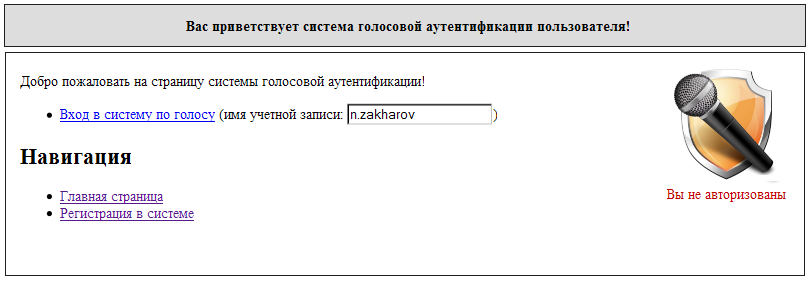
\includegraphics{static_include/main_page.png}}
\caption{Главная страница системы голосовой аутентификации}
\label{fig:main_page}
\end{figure}

При выборе пункта "Регистрация в системе" пользователь автоматически переходит на страницу, которая содержит список требований, удовлетворение которых необходимо для регистрации в системе. Если пользователь авторизован на интернет-ресурсе, на странице присутствует ссылка для перехода к созданию персональной голосовой модели (рисунок~\ref{fig:enrollment_initial_authentificated}). Если пользователь не авторизован, на странице отображается сообщение о необходимости авторизации (рисунок~\ref{fig:enrollment_initial_anonymous}).

\begin{figure}[hbt!]
\center{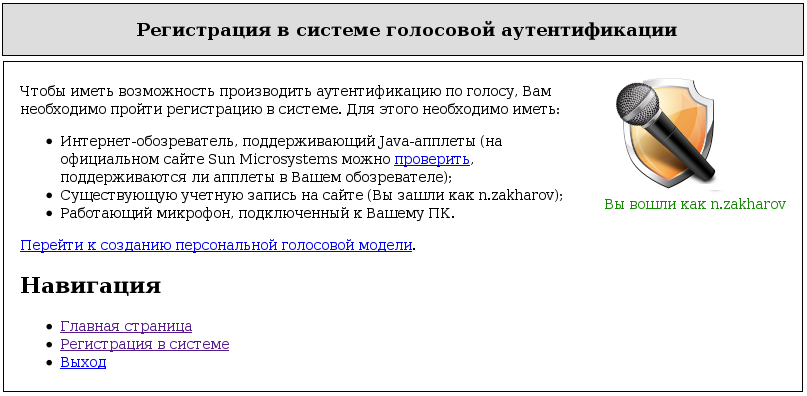
\includegraphics{static_include/enrollment_initial_authentificated.png}}
\caption{Информация о регистрации (пользователь авторизован)}
\label{fig:enrollment_initial_authentificated}
\end{figure}

\begin{figure}[hbt!]
\center{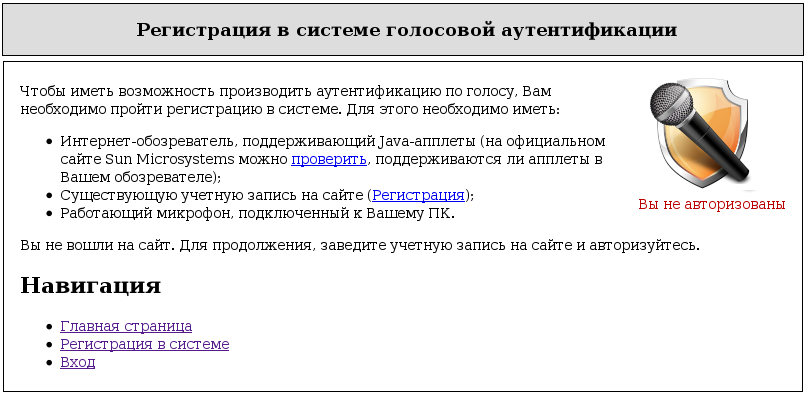
\includegraphics{static_include/enrollment_initial_anonymous.png}}
\caption{Информация о регистрации (пользователь не авторизован)}
\label{fig:enrollment_initial_anonymous}
\end{figure}

\subsubsection{Создание индивидуальной голосовой модели}
\label{sec:manual:enrollment}

В случае выбора ссылки "Перейти к созданию индивидуальной голосовой модели", производится переход к странице с формой, которая представлена на рисунке~\ref{fig:enrollment_created}. В центральной части формы нахоится краткая инструкция по записи образца ключевой фразы. В нижней части находится кнопка "Возврат", при выборе которой происходит автоматический переход на главную страницу системы голосовой аутентификации, и кнопка "Запись".


\begin{figure}[hbt!]
\center{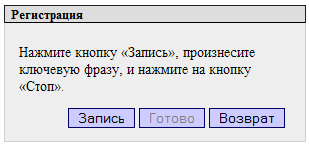
\includegraphics{static_include/enrollment_created.png}}
\caption{Регистрация: инициализация сессии записи}
\label{fig:enrollment_created}
\end{figure}

При выборе кнопки "Запись" начинается запись, и форма  автоматически переходит в состояние, изображенное на рисунке~\ref{fig:enrollment_recording}. В центральной части формы отражается состояние времени записи. В нижней части, заменяя кнопку "Запись", появляется кнопка "Стоп", при нажатии на которую происходит остановка записи.


\begin{figure}[hbt!]
\center{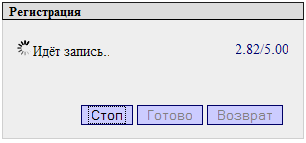
\includegraphics{static_include/enrollment_recording.png}}
\caption{Регистрация: запись голосового образца}
\label{fig:enrollment_recording}
\end{figure}

Если записанный образец слишком короткий, то при выборе кнопки "Стоп", форма переходит в состояние, представленное на рисунке~\ref{fig:enrollment_too_short_to_upload}. В центре формы находится сообщение о длительности образца и рекомендации пользователю. Из данной формы можно перейти в состояние записи голосового образца или вернуться на главную страницу системы голосовой аутентификации.


\begin{figure}[hbt!]
\center{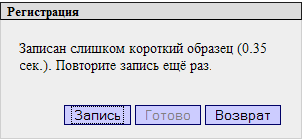
\includegraphics{static_include/enrollment_too_short_to_upload.png}}
\caption{Регистрация: недостаточно данных для отправления}
\label{fig:enrollment_too_short_to_upload}
\end{figure}

Если образец имеет достаточную длину, форма (рисунок~\ref{fig:enrollment_recording}) переходит в состояние, представленное на рисунке~\ref{fig:enrollment_uploading}. В этом состоянии происходит отпрвление записи, что отражается в  центральной части формы, также там отражено время последней записи. 


\begin{figure}[hbt!]
\center{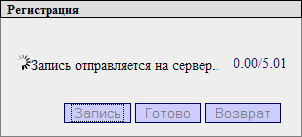
\includegraphics{static_include/enrollment_uploading.png}}
\caption{Регистрация: отправление записи}
\label{fig:enrollment_uploading}
\end{figure}


При возникновении ошибки во время отправления записи, форма переходит в состояние, представленное на рисунке~\ref{fig:enrollment_upload_error}. В центральной части формы расположено сообщение об ошибке и рекомендации пользователю. 


\begin{figure}[hbt!]
\center{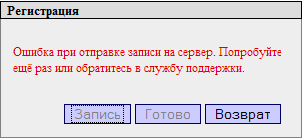
\includegraphics{static_include/enrollment_upload_error.png}}
\caption{Регистрация: ошибка при отправлении записи}
\label{fig:enrollment_upload_error}
\end{figure}



При удачном завершении отправления записи на сервер, форма (рисунок~\ref{fig:enrollment_uploading}) переходит в состояние, изображенное на рисунке~\ref{fig:enrollment_uploaded}. На форме отражается количество, общая длительность записей, и сообшение о состоянии записи. Если пользователь хочет отменить процесс регистрации, необходимо выбрать кнопку "Возврат". Если пользователь хочет продолжить создание голосовой модели, необходимо выбрать кнопку "Запись". Когда пользователь запишит достаточное количество образцов ключевой фразы, становиться активной кнопка "Готово".


\begin{figure}[hbt!]
\center{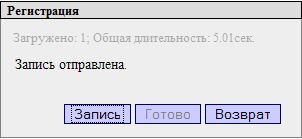
\includegraphics{static_include/enrollment_uploaded.png}}
\caption{Регистрация: запись отправлена}
\label{fig:enrollment_uploaded}
\end{figure}

При выборе кнопки "Готово" начинается процесс обучения модели, и форма переходит в состояние, представленное на рисунке~\ref{fig:enrollment_in_process}. В центральной части формы расположено сообщение о состоянии процесса обучения.

\begin{figure}[hbt!]
\center{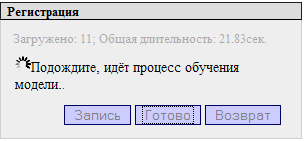
\includegraphics{static_include/enrollment_in_process.png}}
\caption{Регистрация: обучение модели}
\label{fig:enrollment_in_process}
\end{figure}

Если произошла ошибка при обучении модели, форма переходит в состояние, отраженное на рисунке~\ref{fig:enrollment_error_in_learning}. В центре формы отображается сообщение об ошибке и рекомендации пользователю. При возникновении данной ошибки, пользователь может вернуться на главную страницу системы голосовой аутентификации.

\begin{figure}[hbt!]
\center{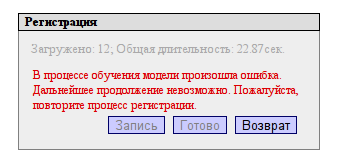
\includegraphics{static_include/enrollment_error_in_learning.png}}
\caption{Регистрация: ошибка во время обучения модели}
\label{fig:enrollment_error_in_learning}
\end{figure}

Если данных для обучения недостаточно, форма (рисунок~\ref{fig:enrollment_in_process}) переходит в состояние, показанное на рисунке~\ref{fig:enrollment_need_more_data}. В центральной части формы отображается сообщение об ошибке и рекомендации пользователю. При возникновении данной ошибки, пользователь может выбрать кнопку "Возврат" или записать дополнительные голосовые данные, выбрав кнопку "Запись".


\begin{figure}[hbt!]
\center{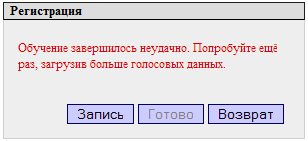
\includegraphics{static_include/enrollment_need_more_data.png}}
\caption{Регистрация: недостаточно данных для обучения модели}
\label{fig:enrollment_need_more_data}
\end{figure}

При удачном завершении обучения модели, регистрация завершается, и форма (рисунок~\ref{fig:enrollment_in_process}) переходит в состояние, показанное на рисунке~\ref{fig:enrollment_success}. Из этого состояния происходит переход на главную страницу системы голосовой аутентификации, что отражается в сообщении.   


\begin{figure}[hbt!]
\center{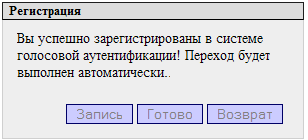
\includegraphics{static_include/enrollment_success.png}}
\caption{Регистрация: успешное завершение обучения модели}
\label{fig:enrollment_success}
\end{figure}

\subsubsection{Аутентификация по голосу}
\label{sec:manual:verification}


Если на главной странице системы голосовой аутентификации не введено имя учётной записи, то при переходе по  ссылке "Вход в систему по голосу", возникает окно с предупреждением (рисунок~\ref{fig:warning_need_login}). Если имя учётной записи введено, производится переход к странице с формой, которая представлена на рисунке~\ref{fig:verification_created}. Центральная часть формы и функция кнопки "Запись" аналогичны описанным в разделе~\ref{sec:manual:enrollment} (рисунок~\ref{fig:enrollment_created}). В нижней части формы находится кнопка "Возврат", при выборе которой, производится переход на главную страницу защищаемого интернет-ресурса.


\begin{figure}[hbt!]
\center{\includegraphics{static_include/need_login.png}}
\caption{Предупреждение о необходимости ввода имени учётной записи}
\label{fig:warning_need_login}
\end{figure}


\begin{figure}[hbt!]
\center{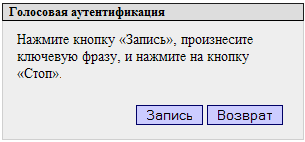
\includegraphics{static_include/verification_created.png}}
\caption{Аутентификация: инициализация сессии записи}
\label{fig:verification_created}
\end{figure}

Процесс записи ключевой фразы для аутентификации аналогичен процессу записи ключевых фраз для создания индивидуальной голосовой модели. Различие заключается в том, что запись производится один раз, после чего начинается процесс аутентификации (рисунок~\ref{fig:verification_in_process}). 


\begin{figure}[hbt!]
\center{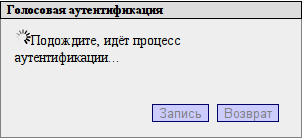
\includegraphics{static_include/verification_in_process.png}}
\caption{Аутентификация: процесс аутентификации}
\label{fig:verification_in_process}
\end{figure}

Если во время аутентификации произошла ошибка , форма переходит в состояние, отраженное на рисунке~\ref{fig:verification_error}. В центре формы отображается сообщение об ошибке и рекомендации пользователю. При возникновении данной ошибки, пользователь может повторить попытку аутентификации, выбрав кнопку "Повтор", или перейти на главную страницу интернет-ресурса, выбрав кнопку "Возврат". 


\begin{figure}[hbt!]
\center{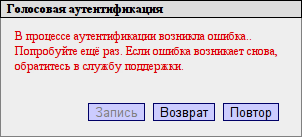
\includegraphics{static_include/verification_error.png}}
\caption{Аутентификация: ошибка во вермя аутентификации}
\label{fig:verification_error}
\end{figure}

Если процесс аутентификации завершился отказом в доступе, форма (рисунок~\ref{fig:verification_in_process}) переходит в состояние, показанное на рисунке~\ref{fig:verification_access_denied}. В центре формы отображается сообщение о состоянии аутентификации и рекомендации пользователю. В нижней части формы находятся кнопки "Возврат" и "Повтор".


\begin{figure}[hbt!]
\center{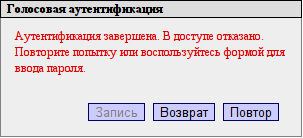
\includegraphics{static_include/verification_access_denied.png}}
\caption{Аутентификация: в доступе отказано}
\label{fig:verification_access_denied}
\end{figure}

Если аутентификация завершается успешно для пользователя (доступ разрешён), происходит автоматический переход на запрошенную страницу, или на страницу, заданную по-умолчанию, администратором интернет-ресурса.  

\subsubsection{Интерфейс администратора}

На главной странице интерфейса администратора представлен список разделов, отвечающих за управление соответствующими объектами системы (рисунок~\ref{fig:admin_main}). Все перечисленные объекты подробно описаны в разделе~\ref{} 

\begin{figure}[hbt!]
\center{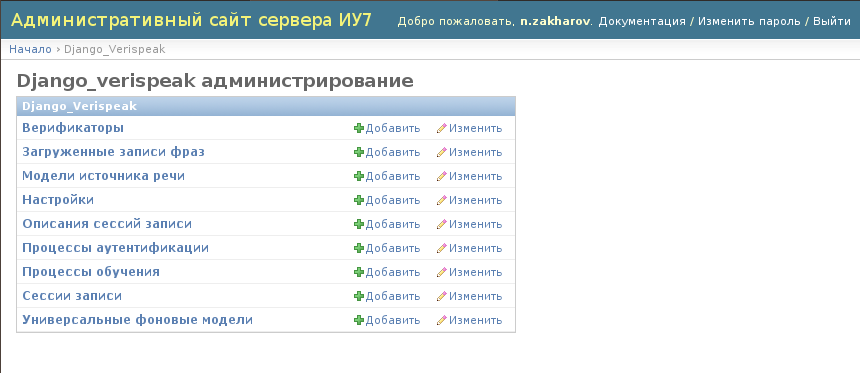
\includegraphics[width=0.8\textwidth]{include/admin_main.png}}
\caption{Главное окно интерфейса администратора}
\label{fig:admin_main}
\end{figure}












